\begin{appendices}
\section {TWIN MUSIC Geometric Acceptance Correction via Efficiency Measurement}
Instead of correcting the limited geometric acceptance of TWIN MUSIC via graphical fitting (see section \ref{sec:geo_corr}) it is also feasible correcting via TWIN MUSIC efficiency measurement. The correction factor is given by:
\begin{equation}\label{eq:twin_eff}
\epsilon_{geo\text{\_}corr} = \frac{N_{MWPC1,MWPC2}}{N_{MWPC1,MWPC2,TWIN}}
\end{equation}
where $N_{MWPC1,MWPC2}$ corresponds to the number of events with a hit in MWPC1 and MWPC2 whereas $N_{MWPC1,MWPC2,TWIN}$ imposes the further condition having a hit in TWIN MUSIC too.\newline
The corresponding correction factor $\epsilon_{geo\text{\_}corr}$ is consequentely applied on all target and empty runs. The resulting corrected charge changing cross section is shown in figure \ref{fig:twim_corr_cc_cs}. 
\begin{figure}[h!]
    \centering
    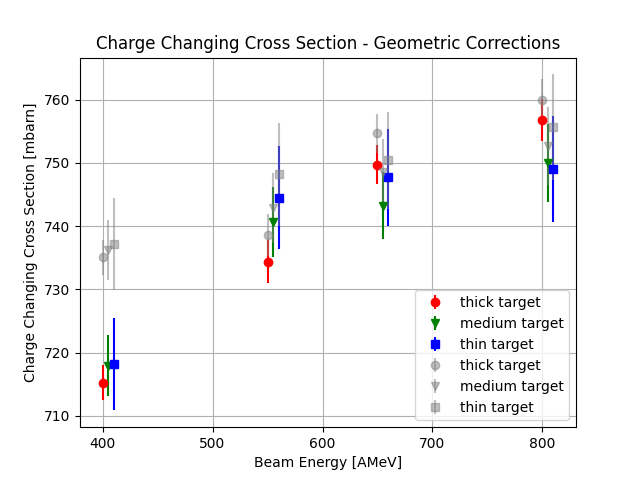
\includegraphics[width=\textwidth,height=8cm,keepaspectratio=true]{Figures/charge_changing_cross_sec_twim_eff_corr.png}
    \caption{
        Charge changing cross section correction due to limited geometric acceptance of TWIN MUSIC via efficieny correction with MWPC1 and MWPC2. In gray: charge changing cross section measurements before applying corrections, as in figure \ref{fig:cccs_gaus_diff_sections}}
    \label{fig:twim_corr_cc_cs}
\end{figure}
The same correction factor can be applied to the total interaction cross section as in figure \ref{fig:twim_corr_tot_cs}. 
\begin{figure}[h!]
    \centering
    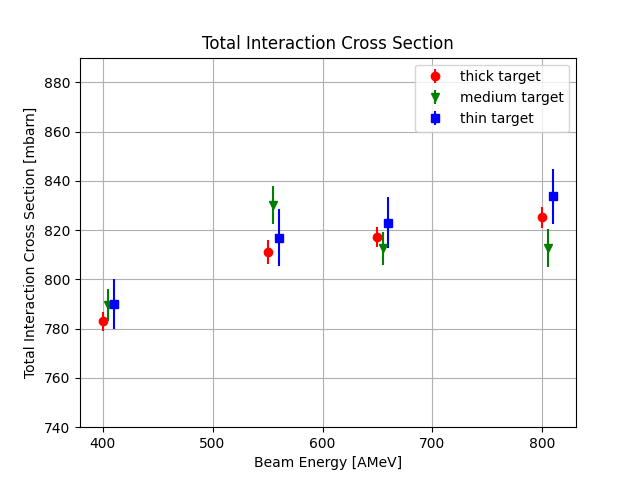
\includegraphics[width=\textwidth,height=12cm,keepaspectratio=true]{Figures/tot_interaction_cs_twim_eff_corr.png}
    \caption{
        Total interaction cross section of $^{12}$C + $^{12}$C using the TWIN MUSIC efficiency correction factor, see equation \ref{eq:twin_eff}, to compensate for the limited geometric acceptance in TWIN MUSIC.}
    \label{fig:twim_corr_tot_cs}
\end{figure}
\newpage


\section{Flight-Path Reconstruction}\label{app:flightpath}
\begin{figure}[h!]
    \centering
    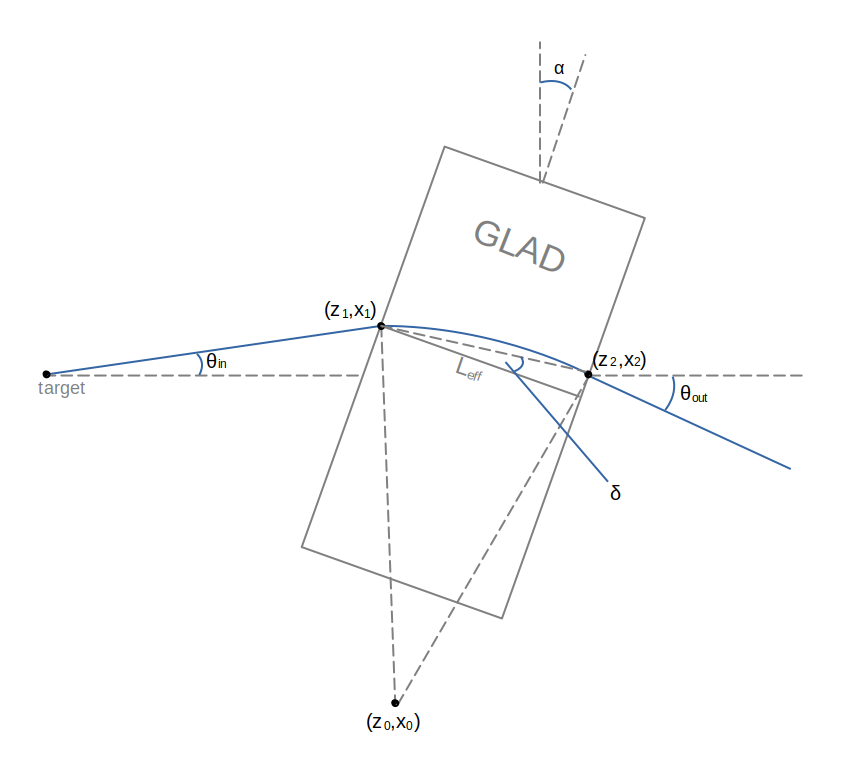
\includegraphics[width=\textwidth]{Figures/drawings_flightpath.png}
    \caption{
        Flightpath reconstruction with reference positions $(x_0,y_0)$, $(x_1,y_1)$ and $(x_2,y_2)$. The GLAD magnet is tilted by $\alpha = 14^{\circ}$.}
    \label{fig:draw_flight}
\end{figure}
The first step in the radius and flightpath reconstruction is expressing the entrance point on the GLAD field $(x_1,y_1)$ and the exit point $(x_2,y_2)$ with the center of the circle path $(x_0,y_0)$ as reference, see figure \ref{fig:draw_flight}:
\begin{align*}
x_1 &= x_0 -r\,cos(90^{\circ}-\theta_i) = x_0 -r\,sin(\theta_i)\\
y_1 &= y_0 + r\,sin(90^{\circ}-\theta_i) = y_0 + r\,cos(\theta_i)\\
\hspace{1cm}
x_2 &= x_0 + r\,cos(90^{\circ}-\theta_o) = x_0 + r\,sin(\theta_o)\\
y_2 &= y_0 + r\,sin(90^{\circ}-\theta_o) = y_0 + r\,cos(\theta_o) 
\end{align*}
The slope $m_1$ of the intersection line between $(x_1,y_1)$ and $(x_2,y_2)$ is given by:
\begin{align*}
m_1 &= \frac{y_2-y_1}{x_2 -x_1} = \frac{cos(\theta_o) - cos(\theta_i)}{sin(\theta_o)+sin(\theta_i)}
\end{align*}
and with the distance between the two points given by:
\begin{align*}
\Delta^2_{i/o} &= r^2 \, \left[(cos\theta_o - cos\theta_i)^2 + (sin\theta_o + sin\theta_i)^2 \right]\\
	       &= 4r^2\,sin^2(\frac{\theta_i}{2} +\frac{\theta_o}{2} )\\
\Rightarrow \Delta_{i/o} &= 2r\,sin(\frac{\theta_i}{2} +\frac{\theta_o}{2})
\end{align*}
To describe the distance between $(x_1,y_1)$ and $(x_2,y_2)$ with the given effective GLAD length $L_{eff}$ ($= 2.06\,m$) the tilting angle $\alpha$ (see figure \ref{fig:draw_flight}) of GLAD in relation to the incoming beam line direction has to be considered. Consequential the angle $\delta$ between the trajectory connecting $(x_1,y_1)$ and $(x_2,y_2)$ and the line parallel to the GLAD width $L_{eff}$ can be determined as:
\begin{flalign*}
tan(\delta) &= |\frac{m_1-m_2}{1+ m_1\cdot m_2}|
\end{flalign*}
with $m_2 = -tan(\alpha)$:
\begin{align*}
\delta = atan \left( \frac{\frac{cos\theta_o - cos\theta_i}{sin\theta_o + sin\theta_i} + tan\alpha}{1-\frac{cos\theta_o - cos\theta_i}{sin\theta_o + sin\theta_i}\,\cdot\, tan\alpha} \right)
\end{align*}
The final relation between $L_{eff}$ and the bending radius $r$ of the fragment within GLAD can be written as:
\begin{equation}
\begin{aligned}
L_{eff} &= 2r\,sin(\frac{\theta_i}{2} + \frac{\theta_o}{2})\,\cdot\, cos\delta \\
	&= 2r\,sin(\frac{\theta_i}{2} + \frac{\theta_o}{2})\,\cdot\,\frac{1}{\sqrt{\delta^2+1}}
\end{aligned}
\end{equation}


\section {second stuff I want to add}\label{appendix_first}
hello here to add, end.
\end{appendices}
